\documentclass[10pt]{beamer}
\usepackage[utf8]{inputenc}
\usepackage[english,russian]{babel}
\usepackage{amsmath,mathrsfs,mathtext}
\usepackage{graphicx, epsfig}
\usepackage{graphicx}
\graphicspath{ {pic/} }
\DeclareGraphicsExtensions{.pdf,.png,.jpg}
\usepackage{caption}
\usepackage{subfig}
\usepackage{amsmath}

\usepackage{multicol}

\usepackage{tikz}

\DeclareMathOperator*{\argmin}{arg\,min}
\DeclareMathOperator*{\argmax}{arg\,max}

\makeatletter
\let\@@magyar@captionfix\relax
\makeatother

\fontsize{10}{15}

\usetheme{Warsaw}
\usecolortheme{sidebartab}
\definecolor{beamer@blendedblue}{RGB}{31,96,49}

%----------------------------------------------------------------------------------------------------------
\title[\hbox to 56mm{Нейросети оптимальной сложности  \hfill\insertframenumber\,/\,\inserttotalframenumber}]
{Автоматическое построение нейросети оптимальной сложности }
\author[В.\,О. Маркин, А.\,Г. Забазнов, Н.\,А. Горян, С.\,Е. Губанов, С.\,К. Таранов]{\large \\Маркин Валерий, Забазнов Антон, Горян Николай, Сергей Губанов, Сергей Таранов, Товкес Артём, Улитин Александр, Криницкий Константин}
\institute{\large
Московский физико-технический институт}

\date{\footnotesize{10 декабря, 2018г.}}
%----------------------------------------------------------------------------------------------------------
\begin{document}
%----------------------------------------------------------------------------------------------------------
\begin{frame}
\titlepage
\end{frame}
%-----------------------------------------------------------------------------------------------------
\begin{frame}{Цель работы}

{\bf Иследуется}\\
\quad
	 Задача выбора структуры нейронной сети.\\
	~\\

{\bf Требуется}\\
\quad
	Найти нейросеть оптимальной сложности.\\
	~\\

{\bf Проблемы}\\
	\begin{itemize}
		\item Большое количество параметров,
		\item Высокая вычислительная сложность оптимизации,
		\item Невозможность использования эвристических и переборных алгоритмов выбора струкутры модели
	\end{itemize}

\end{frame}
%----------------------------------------------------------------------------------------------------------

\begin{frame}{Литература}

	\begin{itemize}
		\item \textit{Yang .Y Hanxiao L., Simonyan K.}\\ Darts: Differentiable architecture search. 2018.
		\item	\textit{Dougal Maclaurin, David Duvenaud, Ryan P. Adams}Gradient-based hyperparameter optimization through reversible learning. In Francis Bach and David Blei, editors, Proceedings of the 32nd International Conference on Machine Learning, volume 37 of Proceedings of Machine Learning Research, pages 2113–2122, Lille, France, 07–09 Jul 2015. PMLR.
	\end{itemize}
	
	\begin{itemize}
		\item \textit{Tommi S. Jaakkol Harald Steck} On the dirichlet prior and bayesian regularization.
% 		\item \textit{LeCun Y., Denker J. , Solla S.}\\ Optimal Brain Damage~// Advances in Neural Information Processing Systems, 1989. Vol. 2. P. 598--605.	
	\end{itemize}
	
\end{frame}
%----------------------------------------------------------------------------------------------------------

\begin{frame}{Постановка задачи}
Рассматриваем задачу классификации.\\
Пусть заданы обучающая и вылидационная выборки:
\[
\mathfrak{D}^{\text{train}} = \{\mathbf{x}_i, y_i\}, \quad i=1,\dots,m^{\text{train}},
\]
\[
\mathfrak{D}^{\text{valid}} = \{\mathbf{x}_i, y_i\}, \quad i=1,\dots,m^{\text{valid}},
\]
 где $\mathbf{x}_i\in\mathbf{X}\subset\mathbb{R}^{\text{n}},\quad y_i\in\mathbf{Y}\subset\mathbb{R}.$\\
~\\
$y\in\mathbf{Y}= \{1,\dots,Z\}$, где $Z$ - количество классов.\\
~\\
Модель задаётся ориентированным графом $\mathbf{G=(V,E)}$\\
~\\
$\mathbf{g}^{i,j} $--- базовые функции ребра $(i, j) $ c весами $\boldsymbol{\gamma}^{i,j}$\\
~\\
Требуется построить такую модель $\mathbf{f}$ c параметрами $\mathbf{W}\in\mathbb{R}^\text{n}$:
\[
\mathbf{f}(\mathbf{x}, \mathbf{W})= \{ \mathbf{f}_i(\mathbf{x}, \mathbf{w}_i)\}_{i=1}^\mathbf{|V|}
\]
где $\mathbf{f_i(x, w_i)}$ - подмодель c параметрами $\mathbf{w}_i$ задаётся как:
\[
\mathbf{f}_i(\mathbf{x}, \mathbf{w}_i)\ = \sum_{j\in adj(i)} \left\langle {\boldsymbol{\gamma}^{i,j}, \mathbf{g}^{i,j}} \right\rangle \mathbf{f}_j(\mathbf{x}, \mathbf{w}_j)\
\].


\end{frame}

%----------------------------------------------------------------------------------------------------------

\begin{frame}{Постановка задачи}

Функция потерь на обучении $L$ и функция потерь на валидации $Q$ задаются как:
\[
L (\mathbf{W}, \mathbf{A}, \boldsymbol{\Gamma})= \log p(\mathbf{Y}^\text{train}|\mathbf{X}^\text{train}, \mathbf{W}, \boldsymbol{\Gamma}) + \boldsymbol{e}^{\mathbf{A}}||\mathbf{W}||^2,
\]
\[
Q (\mathbf{W}, \boldsymbol{\Gamma})= \log p(\mathbf{Y}^\text{valid}|\mathbf{X}^\text{valid}, \mathbf{W}, \boldsymbol{\Gamma}) + \lambda p(\boldsymbol{\Gamma}),
\]
где $\mathbf{A}$ и $\lambda$ --- регуляризационные слагаемые, $p(\boldsymbol{\Gamma})$ - произведение всех произведение вероятностей всех $\boldsymbol{\gamma}^{i,j} \in \boldsymbol{\Gamma}$. \\
~\\
Требуется построить модель классификации $\mathbf{f}$ с параметрами $\mathbf{W}$, доставляющую минимум функции потерь на валидации $Q$.
\[
\mathbf{W}^*( \boldsymbol{\Gamma}) = \argmin_{\mathbf{W}}
L (\mathbf{W}, \boldsymbol{\Gamma})\]

\[
\boldsymbol{\Gamma}^*, \mathbf{A}^* = \min_{\boldsymbol{\Gamma}, \mathbf{A}} Q (\mathbf{W}^*( \boldsymbol{\Gamma}), \boldsymbol{\Gamma})
\]



\end{frame}

%----------------------------------------------------------------------------------------------------------
\begin{frame}{Идея для базовых алгоритмов}
Известно множество всех возможных операций $\mathbf{g}^{i,j} \in \mathbf{G}$. Для перехода к непрерывному пространству таких функций проводится релаксация каждой операции c использованием softmax:


$$\overline{\mathbf{g}}^{(i, j)}(x) = \sum\limits_{\mathbf{g} \in \mathbb{K}}{\frac{exp(\gamma_{\mathbf{g}}^{(i, j)})}{\sum\limits_{\overline{\mathbf{g}} \in \mathbb{K}}exp(\gamma_{\overline{\mathbf{g}}}^{(i, j)})}\mathbf{g}(x)},$$


где $\gamma^{i, j}$ --- вектор, параметризующий комбинацию базовых функций. Таким образом, путём подбора  непрерывных параметров  $\gamma$ осуществляется переход к задаче поиска базовой функции. В конце поиска, каждая комбинация базовых функций $\overline{\mathbf{g}}^{(i, j)}(x) $  меняется на $\mathbf{g}^{(i, j)} = \argmax\limits_{\mathbf{g} \in \mathbb{K}}\gamma_{\mathbf{g}}^{(i, j)}$.\\


\end{frame}

%----------------------------------------------------------------------------------------------------------
\begin{frame}{Описание эксперимента}
В качестве выборки использовалась выборка изображений CIFAR-10. Основным критерием качества выступал 
$$Accuracy = \frac{1}{m^\text{valid}}\sum_{\mathbf{x}, y \in \mathfrak{D}^\text{valid}} I(\mathbf{f}(\mathbf{x}), y)$$
В качестве регуляризации использовались:\\
\begin{enumerate}
    \item Слабая регуляризация(Дирихле с параметром $\alpha = 1$).\\
    \item Меняющейся регуляризация(Дирихле с параметром $\alpha$, меняющимся на каждой эпохи в интервале $(10^{-30}; 1)$).\\
    \item Сильной регуляризацией(распределение Дирихле с параметром  $\alpha= 10^{-30}$).\\
\end{enumerate}
\end{frame}

%----------------------------------------------------------------------------------------------------------
% \begin{frame}{Устойчивость модели к шуму в параметрах модели}

% \centering
% 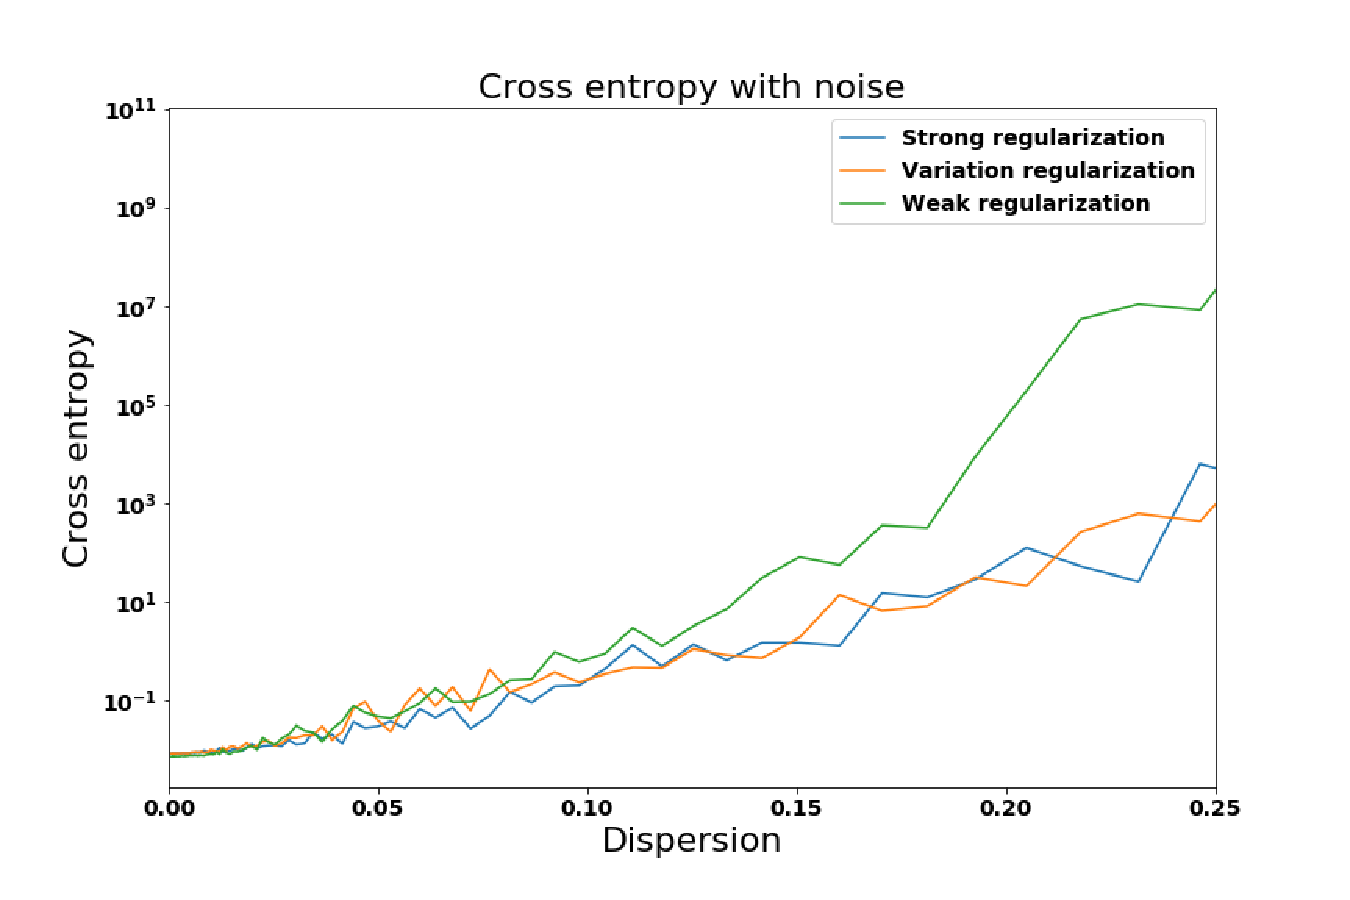
\includegraphics[width=1\linewidth]{slides_ce_noise_params_graph.pdf}
% \caption{}
% \label{}

% \end{frame}

% \begin{frame}{Устойчивость модели к шуму в параметрах модели}

% \centering
% 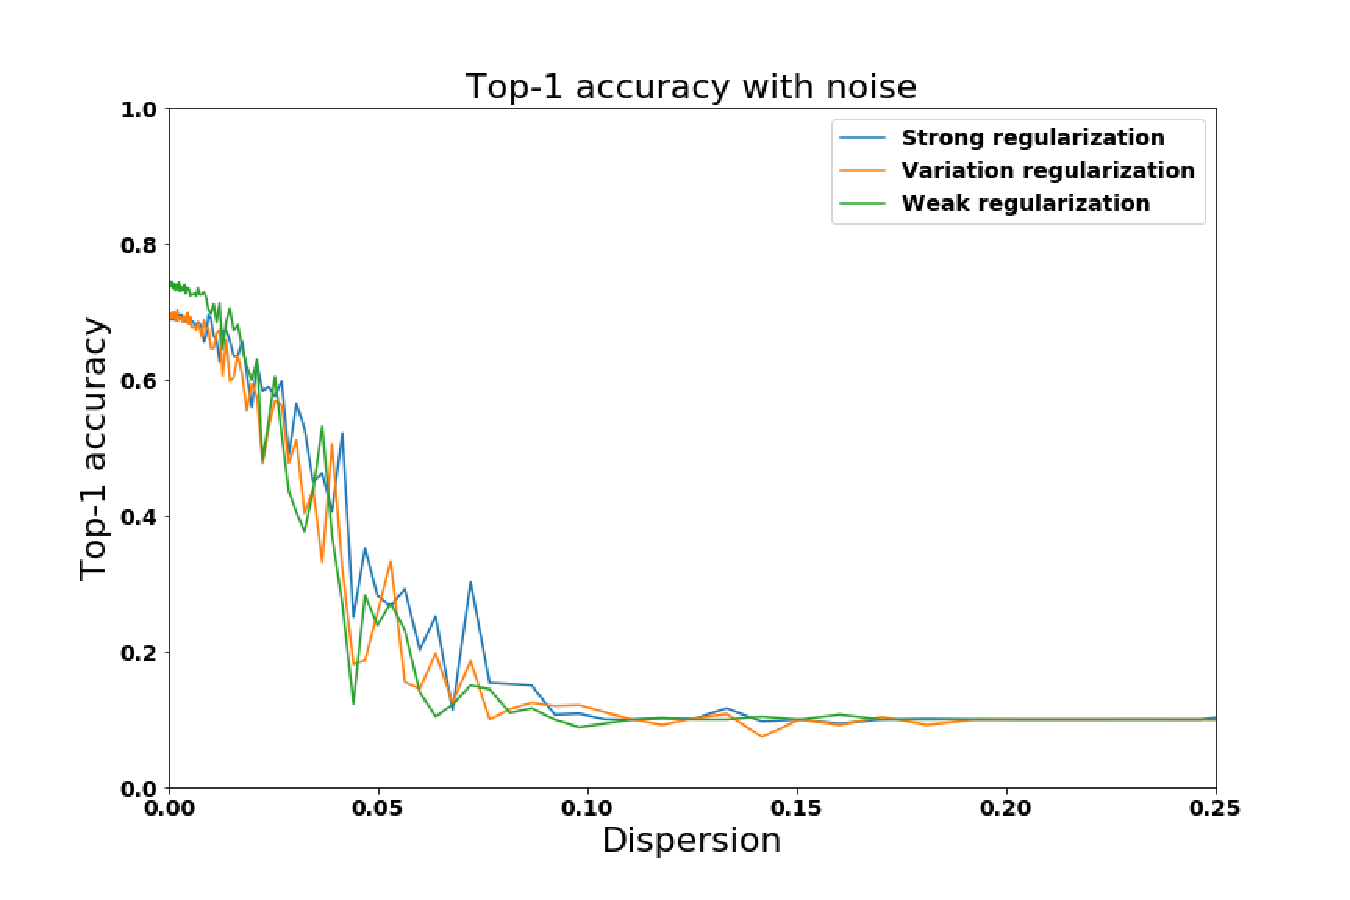
\includegraphics[width=1\linewidth]{slides_t1_noise_params_graph.pdf}
% \caption{}
% \label{}

% \end{frame}

% \begin{frame}{Устойчивость модели к шуму в параметрах модели}

% \centering
% 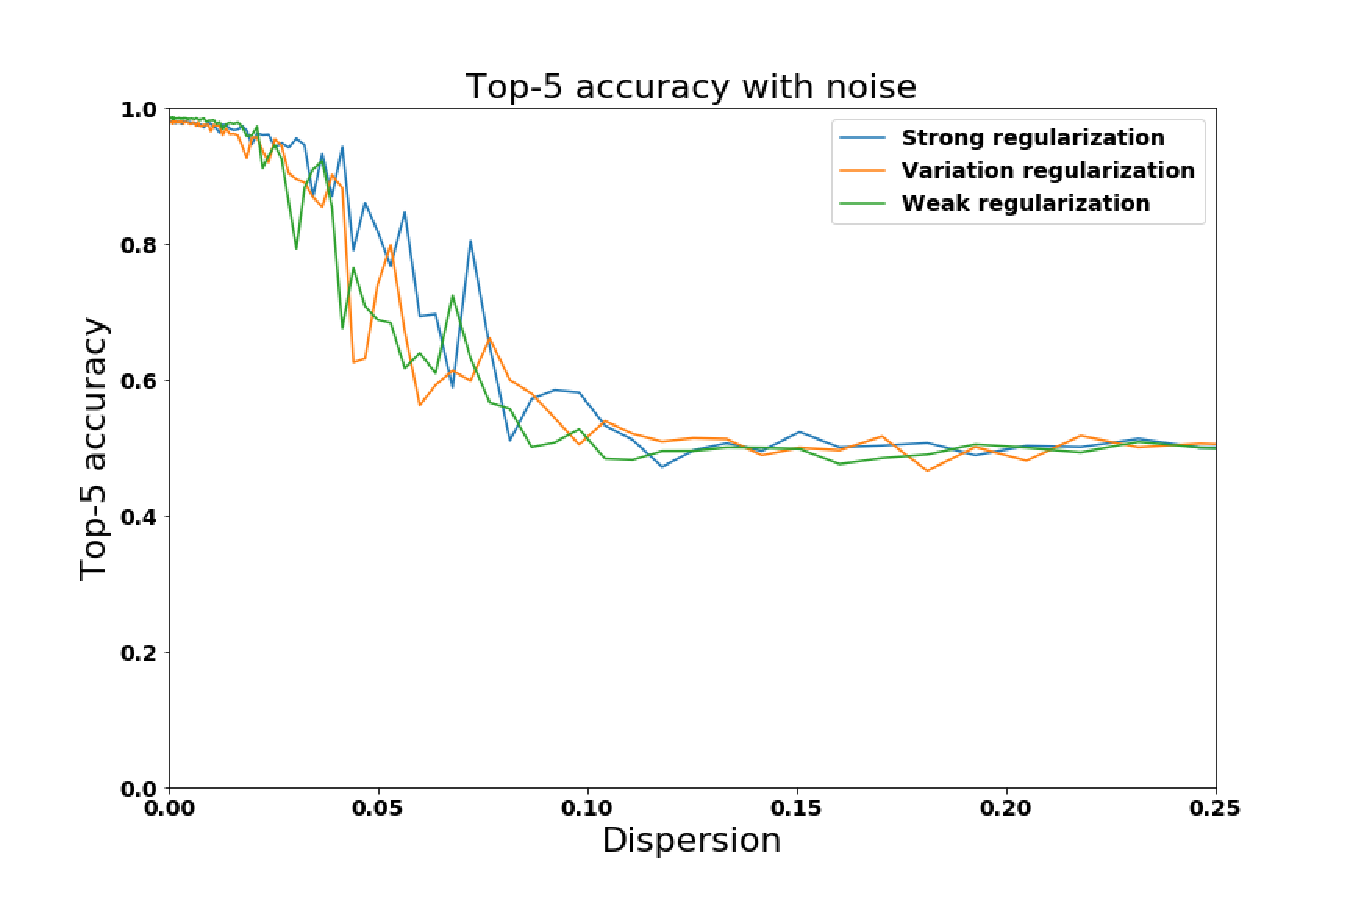
\includegraphics[width=1\linewidth]{slides_t5_noise_params_graph.pdf}
% \caption{}
% \label{}

% \end{frame}

% \begin{frame}{Устойчивость модели к шуму в данных}

% \centering
% 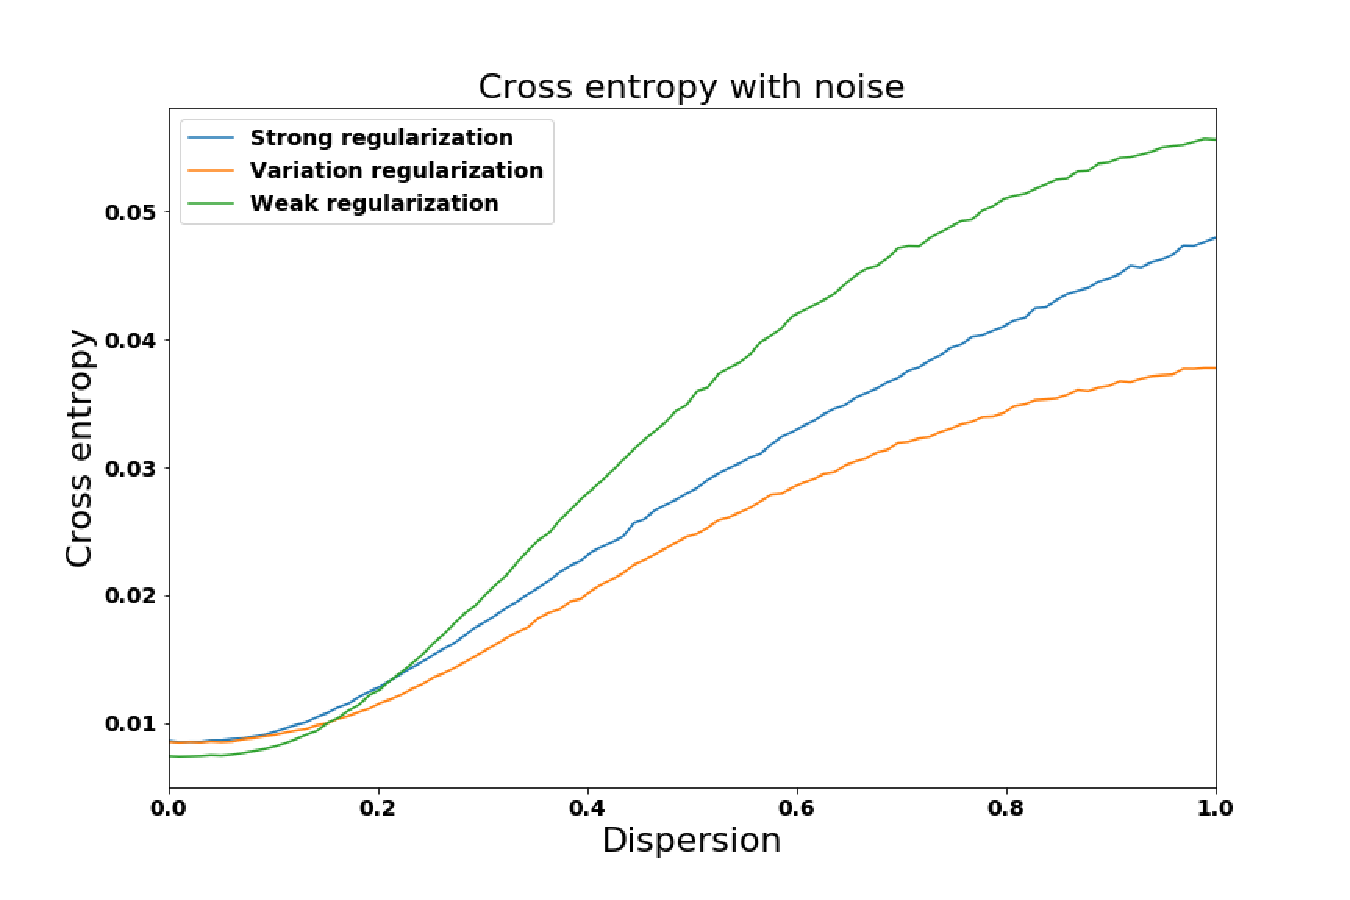
\includegraphics[width=1\linewidth]{slides_ce_noise_graph.pdf}
% \caption{}
% \label{}

% \end{frame}

\begin{frame}{Устойчивость модели к шуму в данных}

\centering
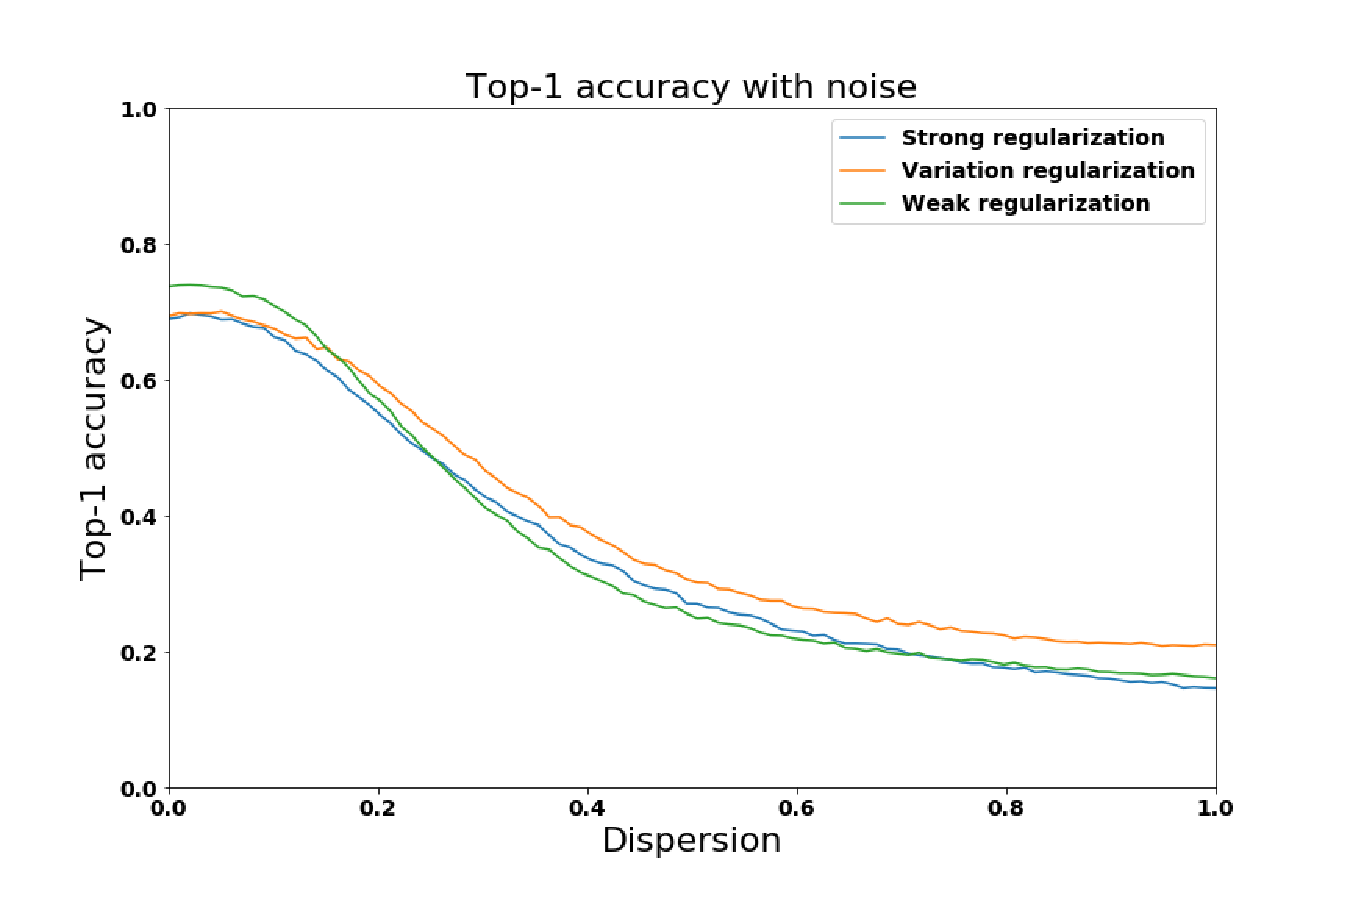
\includegraphics[width=1\linewidth]{slides_t1_noise_graph.pdf}
\caption{}
\label{}

\end{frame}

\begin{frame}{Устойчивость модели к шуму в данных}

\centering
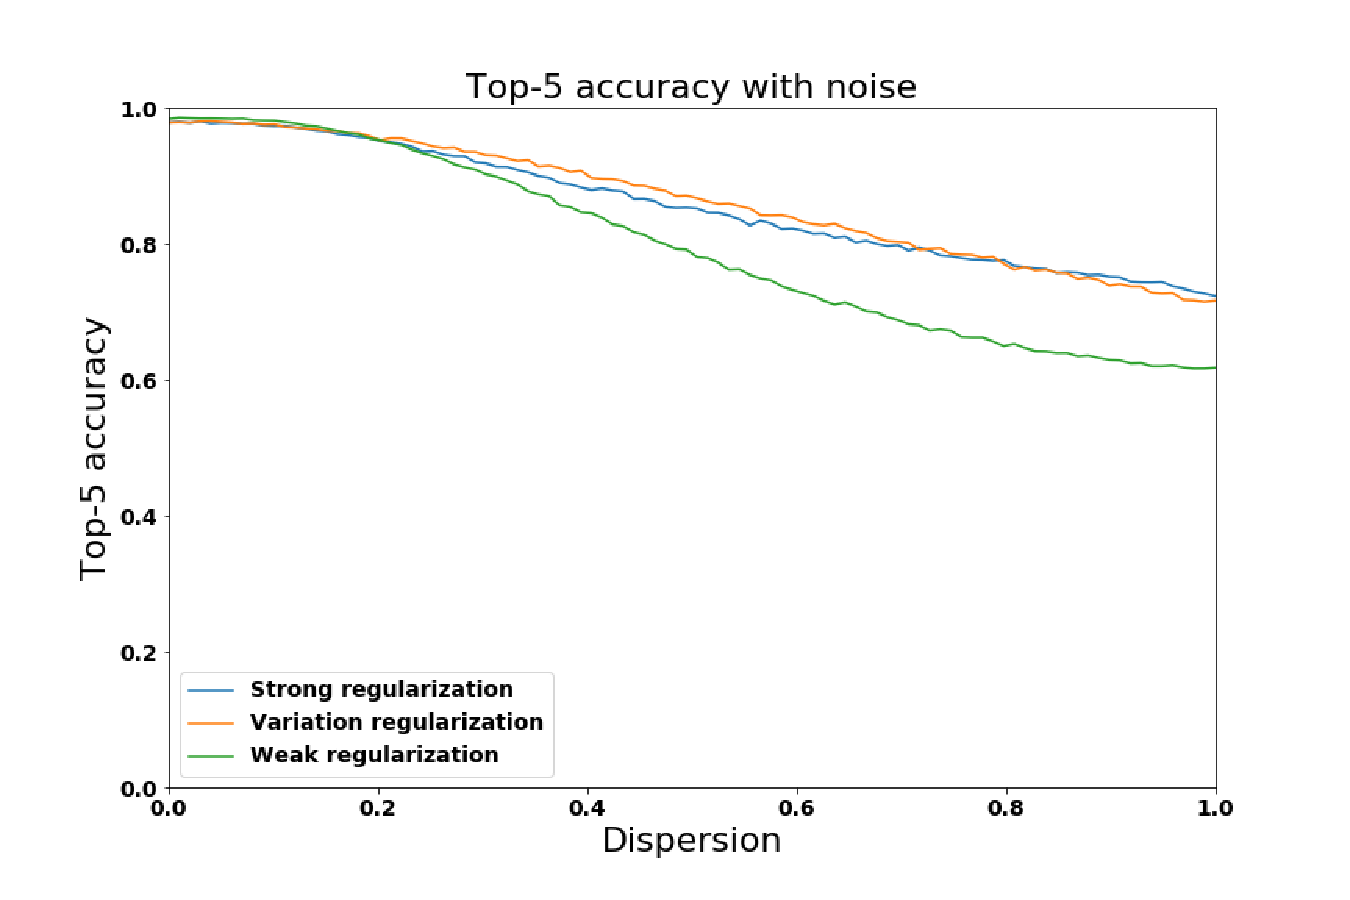
\includegraphics[width=1\linewidth]{slides_t5_noise_graph.pdf}
\caption{}
\label{}

\end{frame}

%!!!!!!!!!!!!!!!!!!!!!!!!1
\begin{frame}{Динамика изменения структурных параметров в процессе обучения}

\begin{minipage}[h]{0.31\linewidth}
\center{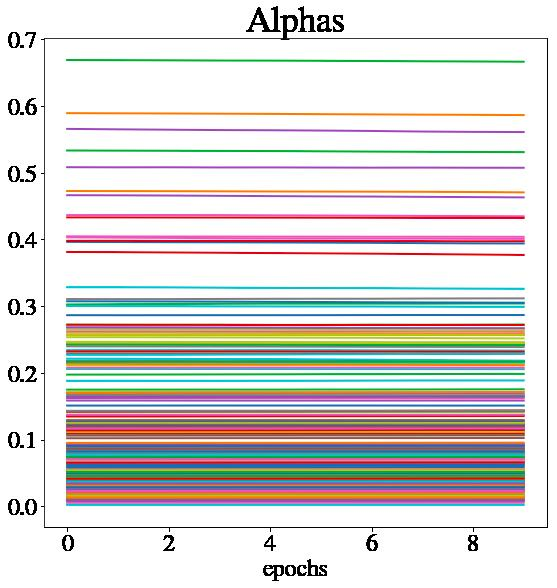
\includegraphics[width=1\linewidth]{alphas_weak.jpeg} \\ слабая \n регуляризация}
\end{minipage}
\begin{minipage}[h]{0.31\linewidth}
\center{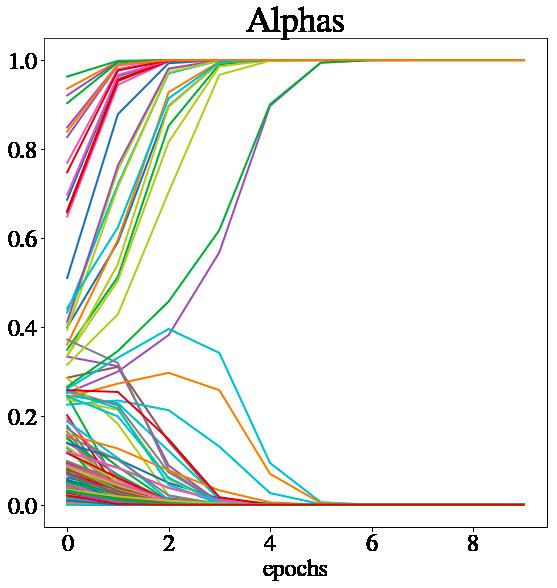
\includegraphics[width=1\linewidth]{alphas_strong.jpeg} \\ сильная регуляризация}
\end{minipage}
\begin{minipage}[h]{0.31\linewidth}
\center{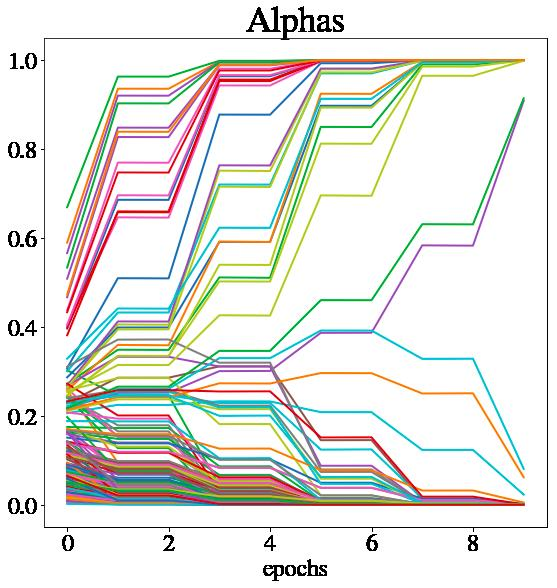
\includegraphics[width=1\linewidth]{alphas_variable.jpeg} \\ вариационная регуляризация}
\end{minipage}
% {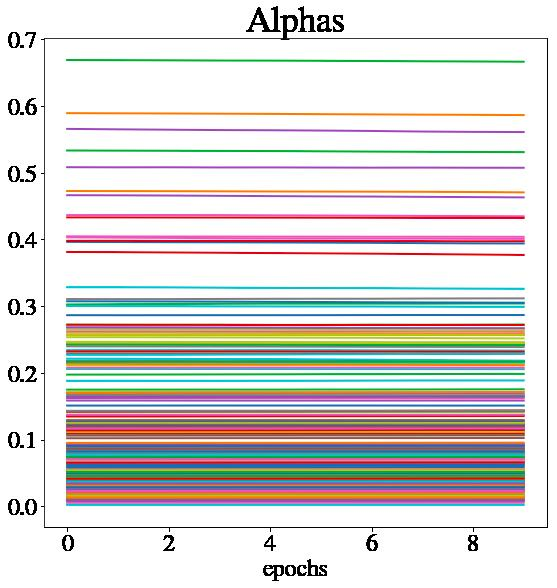
\includegraphics[width=0.5\textwidth]{alphas_weak.jpeg}}
% \subfloat[2 режим] {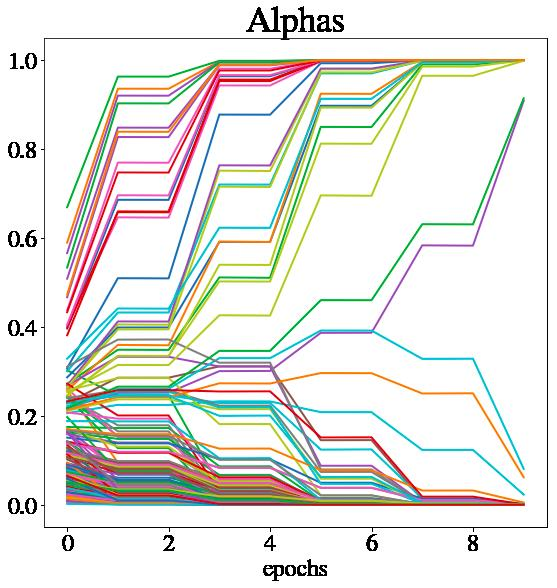
\includegraphics[width=0.5\textwidth]{alphas_variable.jpeg}}\\
% \subfloat[3 режим] {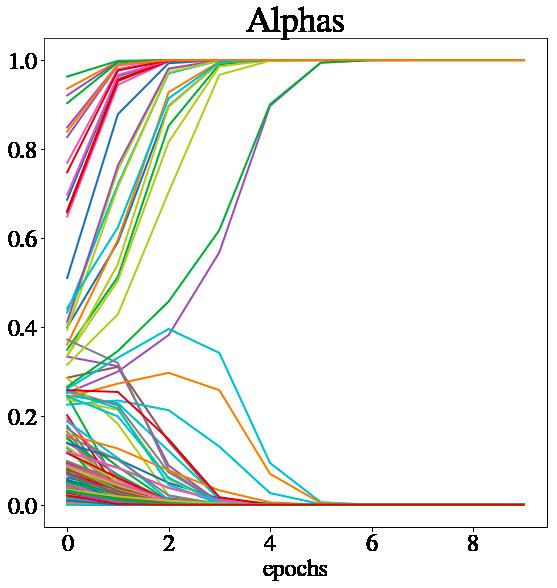
\includegraphics[width=0.5\textwidth]{alphas_strong.jpeg}}
\caption{}
\label{}

\end{frame}

% \begin{frame}{Динамика изменения структурных параметров в процессе обучения для слабой регуляризации}

% \centering
% 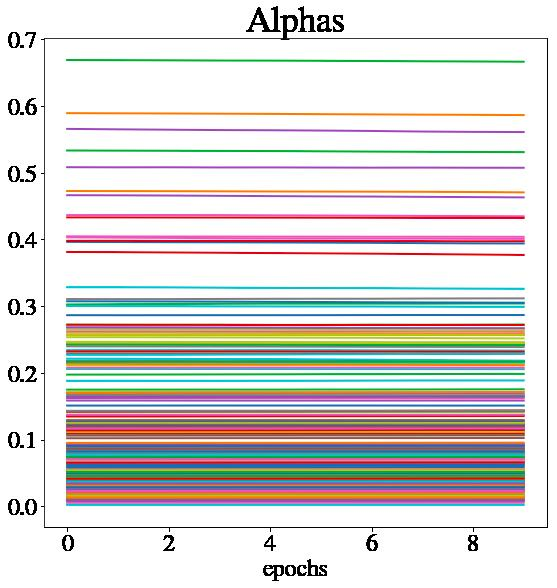
\includegraphics[width=0.6\linewidth, hight=1\textwidth    ]{alphas_weak.jpeg}
% \caption{}
% \label{}


% \end{frame}

% \begin{frame}{Динамика изменения структурных параметров в процессе обучения для сильной регуляризации}

% \centering
% 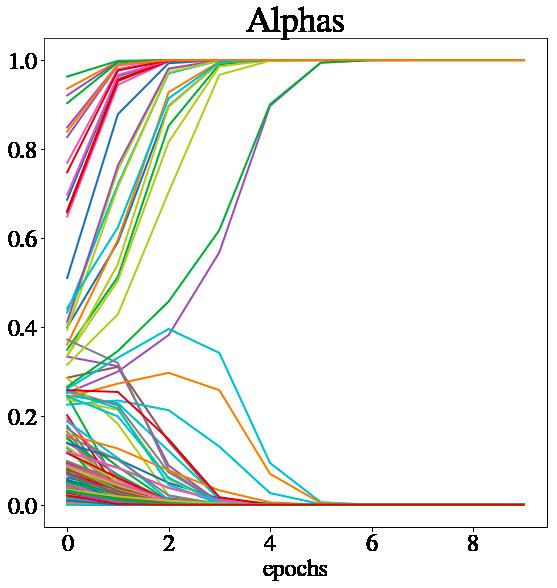
\includegraphics[width=0.6\linewidth]{alphas_strong.jpeg}
% \caption{}
% \label{}

% \end{frame}

% \begin{frame}{Динамика изменения структурных параметров в процессе обучения для вариационной регуляризации}

% \centering
% 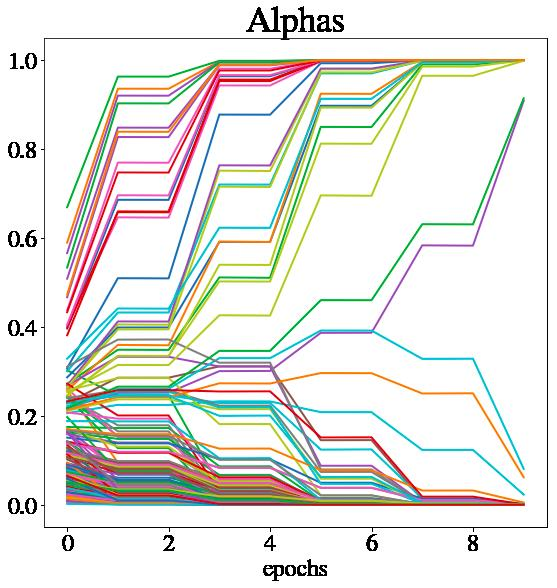
\includegraphics[width=0.6\linewidth]{alphas_variable.jpeg}
% \caption{}
% \label{}

% \end{frame}

%-------------------------------------------------------------------------------------------------------------
\begin{frame}{Вывод}

\begin{itemize}
	\item Проведен эксперимент по регялиразции структуры нейронной сети на выборке CIFAR-10
	\item Эксперименты показали, что структура нейронной сети вырождается в дискретную при использовании регуляризации
	\item Эксперимент показал, что оптимизация подвержена застреванию в стационарных точках пространства структурных параметров
\end{itemize}

{\bf Планируется}\\
	\begin{itemize}
		\item Предложить метод регуляризации, позволяющий избегать застревания в стационарных точках
	\end{itemize}

\end{frame}
%----------------------------------------------------------------------------------------------------------




\end{document}